\documentclass[tikz,border=4mm]{standalone}
      \usepackage{tikz}
      \usetikzlibrary{arrows.meta,positioning,calc,shapes.geometric}
      \begin{document}
      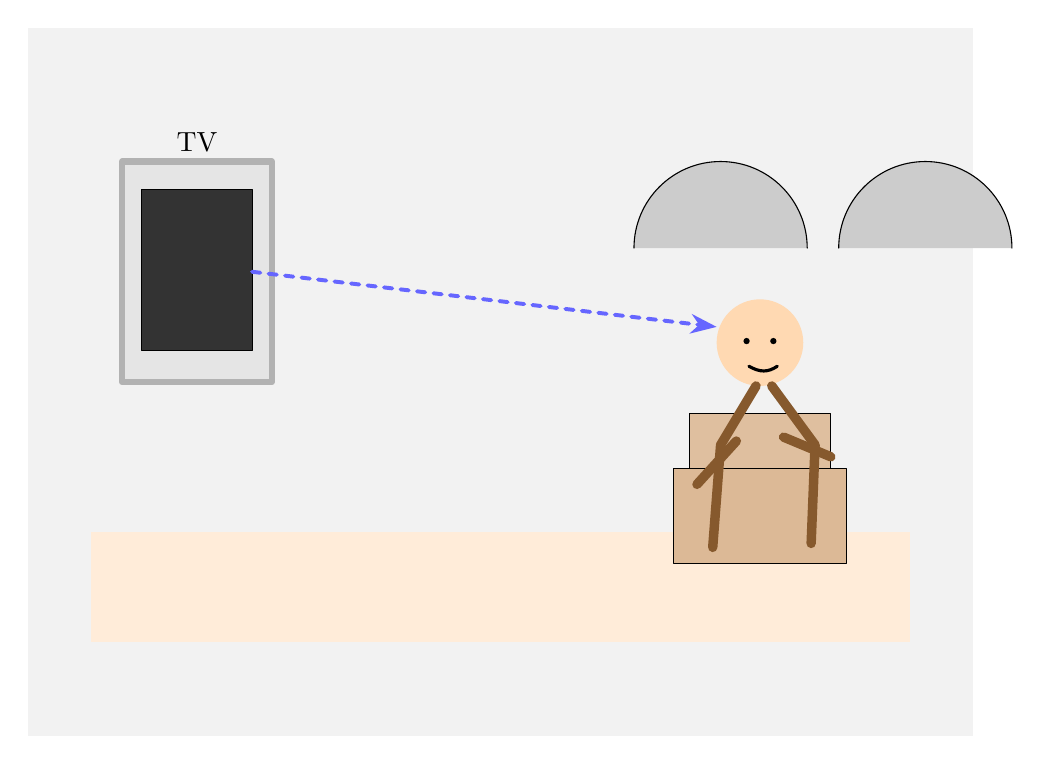
\begin{tikzpicture}[>=Stealth, line cap=round, line join=round]

\fill[fill=gray!10] (0,0) rectangle (12,9);
\fill[fill=orange!15] (0.8,1.2) rectangle (11.2,2.6);
\draw[fill=gray!20, draw=gray!60, line width=0.08cm] (1.2,4.5) rectangle (3.1,7.3);
\draw[fill=black!80] (1.45,4.9) rectangle (2.85,6.95);
\node[above] at (2.15,7.3) {TV};
\draw[fill=brown!50] (8.4,3.2) rectangle (10.2,4.1);
\draw[fill=brown!55] (8.2,2.2) rectangle (10.4,3.4);
\fill[fill=orange!30] (9.3,5) circle (0.55);
\draw[line width=0.12cm, brown!70!black] (9.25,4.45) -- (8.8,3.7) -- (8.7,2.4);
\draw[line width=0.12cm, brown!70!black] (9.45,4.45) -- (10.0,3.7) -- (9.95,2.45);
\draw[line width=0.12cm, brown!70!black] (9.0,3.75) -- (8.5,3.2);
\draw[line width=0.12cm, brown!70!black] (9.6,3.8) -- (10.2,3.55);
\fill (9.13,5.02) circle (0.04);
\fill (9.47,5.02) circle (0.04);
\draw[line width=0.04cm] (9.16,4.7) .. controls (9.3,4.62) and (9.4,4.62) .. (9.52,4.7);
\draw[fill=gray!40] (7.7,6.2) arc[start angle=180, end angle=0, x radius=1.1, y radius=1.1];
\draw[fill=gray!40] (10.3,6.2) arc[start angle=180, end angle=0, x radius=1.1, y radius=1.1];
\draw[blue!60, dashed, line width=0.05cm, ->] (2.85,5.9) -- (8.75,5.2);

      \end{tikzpicture}
      \end{document}
